\documentclass[tikz,border=10pt]{standalone}

\usepackage{tikz}
\usetikzlibrary{positioning}
\usetikzlibrary{shapes,arrows,backgrounds,fit,shapes.geometric,calc}
\usetikzlibrary{pgfplots.groupplots}
\usepackage{pgfplots}
\usepackage{pgfplotstable}
\usepackage{listings}
\usepackage{lstautogobble}
\usepackage{color}

\lstset{
    language=[ANSI]C++,
    basicstyle=\small\ttfamily,
    identifierstyle=\color{black}\small\ttfamily,
    keywordstyle=\color{red}\small\ttfamily,
    commentstyle=\color{green!30!black}\bf\small\ttfamily,
    breaklines=true
}

\tikzset{
    %Define standard arrow tip
    >=stealth',
    % Define arrow style
    pil/.style={
           ->,
           thick,
           shorten <=2pt,
           shorten >=2pt,}
}

\newcommand{\nodewidth}{1cm}
\newcommand{\nodeheight}{1cm}
\newcommand{\memwidth}{12cm}
\newcommand{\memheight}{2cm}

\begin{document}
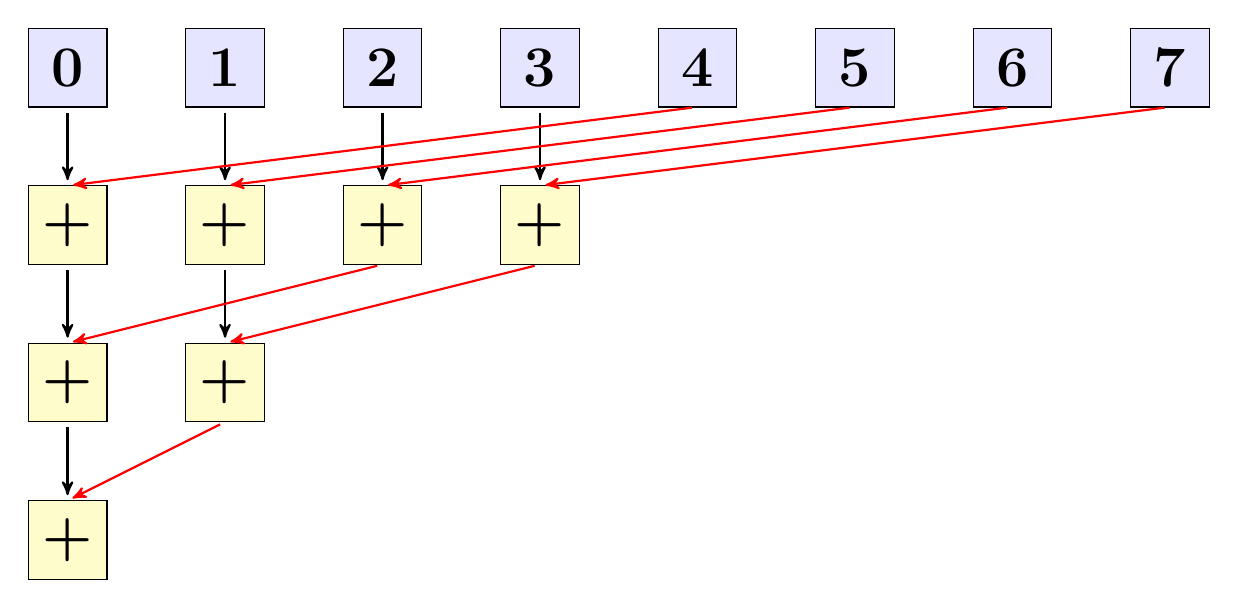
\begin{tikzpicture}[x=0cm, y=0cm, node distance=0 cm,outer sep = 0pt]
\tikzstyle{core}=[draw, rectangle,  minimum height=\nodeheight, minimum width=\nodewidth, fill=blue!10,anchor=north west]
\tikzstyle{res}=[draw, rectangle,  minimum height=\nodeheight, minimum width=\nodewidth, fill=yellow!20,anchor=north west]

\node[core] (core0) at(0,0) {\huge\textbf{0}};
\node[core] (core1) [right = 1cm of core0] {\huge\textbf{1}};
\node[core] (core2) [right = 1cm of core1] {\huge\textbf{2}};
\node[core] (core3) [right = 1cm of core2] {\huge\textbf{3}};
\node[core] (core4) [right = 1cm of core3] {\huge\textbf{4}};
\node[core] (core5) [right = 1cm of core4] {\huge\textbf{5}};
\node[core] (core6) [right = 1cm of core5] {\huge\textbf{6}};
\node[core] (core7) [right = 1cm of core6] {\huge\textbf{7}};

\node[res] (one0) [below = 1cm of core0] {\huge\textbf{+}};
\node[res] (one1) [below = 1cm of core1] {\huge\textbf{+}};
\node[res] (one2) [below = 1cm of core2] {\huge\textbf{+}};
\node[res] (one3) [below = 1cm of core3] {\huge\textbf{+}};

\path[pil,->] (core0.south)  edge (one0.north);
\path[pil,->] (core1.south)  edge (one1.north);
\path[pil,->] (core2.south)  edge (one2.north);
\path[pil,->] (core3.south)  edge (one3.north);
\path[pil,->,red] (core4.south)  edge (one0.north);
\path[pil,->,red] (core5.south)  edge (one1.north);
\path[pil,->,red] (core6.south)  edge (one2.north);
\path[pil,->,red] (core7.south)  edge (one3.north);

\node[res] (two0) [below = 1cm of one0] {\huge\textbf{+}};
\node[res] (two1) [below = 1cm of one1] {\huge\textbf{+}};

\path[pil,->] (one0.south)  edge (two0.north);
\path[pil,->] (one1.south)  edge (two1.north);
\path[pil,->,red] (one2.south)  edge (two0.north);
\path[pil,->,red] (one3.south)  edge (two1.north);

\node[res] (result) [below = 1cm of two0] {\huge\textbf{+}};

\path[pil,->] (two0.south)  edge (result.north);
\path[pil,->,red] (two1.south)  edge (result.north);

\end{tikzpicture}

\end{document}

